\documentclass[11pt, a4paper]{article}

\usepackage{graphicx}
\usepackage[english]{babel}
\usepackage[utf8x]{inputenc}
\usepackage{amsmath}
\usepackage[a4paper,top=3cm,bottom=2cm,left=2cm,right=2cm,marginparwidth=1.75cm]{geometry}
\usepackage{amssymb}

\graphicspath{ {./images} }
\newcommand*{\qed}{\hfill\ensuremath{\quad\square}}%
\newcommand*{\rad}{\ensuremath{\,\text{rad}}}
\newcommand*{\R}{\ensuremath{\mathbb{R}}}

\makeatletter
\renewcommand*\env@matrix[1][*\c@MaxMatrixCols c]{%
  \hskip -\arraycolsep
  \let\@ifnextchar\new@ifnextchar
  \array{#1}}
\makeatother

\newtheorem{theorem}{Theorem}

\begin{document}

\setcounter{section}{8}
\section{Lecture 9: Subspaces}
\subsection{Definition of a subspace}
A subspace in $\mathbb{R}^n$ is a set of vectors $W$ where:
\begin{enumerate}
  \item $\vec{0} \in W$
  \item if $\vec{u}$, $\vec{v}$ $\in W$, then $\vec{u} + \vec{v} \in W$
  \item if $\vec{u} \in W$ and $c \in \mathbb{R}$, then $c\vec{u} \in W$
\end{enumerate}

Items 2 in the list can also be formulated differently as: All linear combinations of the vectors that span $W$ will
also be in $W$.

\begin{theorem}
  The span of a set of vectors $\{ \vec{v}_1, \cdots, \vec{v}_n   \}\in \mathbb{R}^m$ is a subspace of $\mathbb{R}^m$.
\end{theorem}
Because of theorem 1 we can conclude that $\text{Span}\{ W\} \in W$.


\subsection{Null space and column space}
The Null space Nul $A$ is the set of all solutions to the homogeneous equation $A\vec{x} = \vec{0}$.
To prove that the Nul space is indeed a subspace we have to prove that it statisfy the 3 criteria of a 
subspace noted earlier.
\begin{gather}
  \text{let: } \vec{v},\vec{w} \in \text{Nul } A, c\in \mathbb{R} \notag\\
  1)\; A\vec{0} = \vec{0}\\
  2)\; A(\vec{v} + \vec{w}) = A\vec{v} + A\vec{w} = A\vec{0} + A\vec{0} = \vec{0}\\
  3)\; A(c\vec{v}) = cA\vec{v} = c\cdot \vec{0} = \vec{0} \qed
\end{gather}

The column space Col $A$ of a matrix $A$ is the span of the columns of $A$. 

\begin{gather*}
  \begin{bmatrix}[cc]
    a & b\\
    c & d\\
  \end{bmatrix}
  \text{then Col $A$ will be:}\\
  \text{Span} \begin{Bmatrix} \begin{pmatrix} a\\ c\\ \end{pmatrix}, \begin{pmatrix} b\\ d\\ \end{pmatrix} \end{Bmatrix}
\end{gather*}
This can be written down more generally as:
\begin{gather*}
  \text{Col } A = \text{Span } \{ \vec{a}_1, \vec{a}_2, \cdots, \vec{a}_n \} = \{ x_1\vec{a}_1 + \cdots + x_n\vec{a}_n | x_1, \cdots, x_n \in \R \} 
\end{gather*}

Note that $x_1\vec{a}_1 + \cdots + x_n\vec{a}_n = \vec{b}$ or written in terms
of a matrix vector product $A\vec{x} = \vec{b}$ is consistent if $\vec{b} \in \text{Col }A$.

\begin{theorem}
  Nul $A$ of an $m \times n$ matrix $A$ is a subspace of $\R^n$
\end{theorem}

\begin{theorem}
  Col $A$ of an $m \times n$ matrix is a subspace of $\R^m$.
\end{theorem}

\subsection{Null Space example}
let $A = \begin{bmatrix} 1 & 2 & 3\\ 0 & 2 & 1\\ \end{bmatrix}$, $\vec{x} =\begin{pmatrix} x_1 \\ x_2 \\ x_3\\ \end{pmatrix}$

\begin{gather*}
  A\vec{x} = \vec{0}\\
  \begin{bmatrix} 1 & 2 & 3\\ 0 & 2 & 1\\ \end{bmatrix}
    \cdot
  \begin{pmatrix} x_1 \\ x_2 \\ x_3\\ \end{pmatrix}
    =
  \begin{pmatrix} 0 \\ 0 \\ 0\\ \end{pmatrix}\\
  \begin{bmatrix}[ccc|c]
    1 & 2 & 3 & 0\\
    0 & 2 & 1 & 0\\
  \end{bmatrix}
  \sim
  \begin{bmatrix}[ccc|c]
    1 & 0 & 2 & 0\\
    0 & 1 & \frac{1}{2} & 0\\
  \end{bmatrix}\\
  \begin{cases}
    x_1 = -2x_3\\
    x_2 = -\frac{1}{2}x_3\\
    x_3 = \text{free}
  \end{cases}
  \Rightarrow
  \begin{pmatrix} x_1 \\ x_2 \\ x_3\\ \end{pmatrix}
    =
    x_3 \cdot \begin{pmatrix} -2 \\ -\frac{1}{2} \\ 1\\ \end{pmatrix}\\
  \text{Thus: } \text{Nul } A = \text{Span} \begin{Bmatrix} \begin{pmatrix} -2 \\ -\frac{1}{2} \\ 1\\ \end{pmatrix} \end{Bmatrix}
\end{gather*}

\begin{figure}[h]
  \centerline{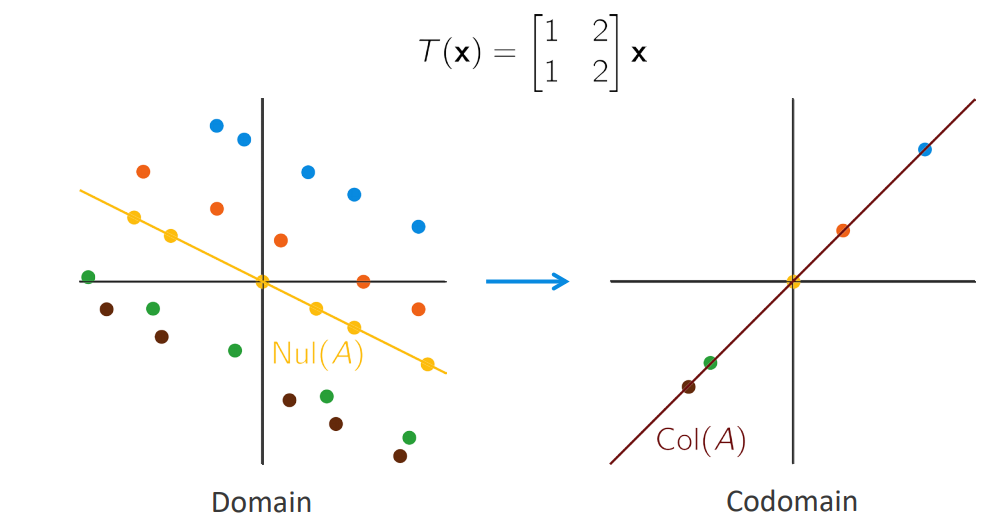
\includegraphics[width=10cm]{images/Subspaces.png}}
  \caption{A visual example of column and null spaces}
\end{figure}


\subsection{Basis of a subspace}
A basis of a subspace $W$ is defined as the set of vectors $\{ \vec{v}_1, \cdots, \vec{v}_p \}$ in $W$ which
is both linearly independent and spans $W$. This is not a unique set of vectors; A subspace can have
many different bases.

\begin{theorem}
  Different bases of the same subspace $W$ of $\mathbb{R}^n$ will have the same number of vectors.
\end{theorem}



\end{document}